\documentclass[a4paper,twocolumn,10pt]{article}

\usepackage{eurosis}
\usepackage{url}
\usepackage{natbib}

\usepackage[pdftex]{graphicx}
\graphicspath{{images/}}

\begin{document}

\title{EDUCATIONAL APPROACH IN FINDING GENERAL FORMULAS FOR SOLUTION OF TWISTY PUZZLES}

\author{Gergana Mateeva, Petar Tomov, Kalin Kopanov, Velizar Varbanov, Todor Balabanov \\
Institute of Information and Communication Technologies \\
Bulgarian Academy of Sciences \\
email: \texttt{gergana.mateeva|petar.tomov|kalin.kopanov|velizar.varbanov|todor.balabanov} \\ 
\texttt{@iict.bas.bg}}

\date{}

\maketitle

\thispagestyle{empty}

\keywords{Combination Puzzle, Formal Grammars, Formulas Generation}

\begin{abstract}
The difficulty in solving twisty puzzles like the Rubik's Cube and Hungarian Rings is determining the precise sequence of moves required to attain a specific objective. These puzzles commence in a state where the elements, such as colored stickers or rings, appear intricate and seemingly haphazard. The objective is to rearrange them into a particular pattern or configuration. Solving the puzzle involves manipulating the elements through diverse moves, such as rotating different layers of the Rubik's Cube or adjusting the position of rings in the Hungarian Rings. Each move exerts a distinct influence on the configuration of the puzzle. Solvers frequently use trial and error, experimenting with various move sequences to observe their effects. The solution necessitates a blend of spatial reasoning, pattern recognition, and strategic thinking. Proficient solvers often utilize algorithmic sequences of moves tailored to achieve specific outcomes. These algorithms are crafted through experience and analysis of the puzzle's mechanics. Efficient solving entails solving with the fewest possible moves. For instance, speedcubers strive to solve the Rubik's Cube quickly by employing optimized algorithms. To commit these algorithms to memory, solvers may utilize logical deduction to assess the puzzle's state and make informed decisions about the subsequent moves. The present research delves into developing universal formulas for a puzzle known as Fish Rings.
\end{abstract}

\section{INTRODUCTION}

Combinatorial puzzles are a type of game that consists of groups of connected pieces. This connectivity distinguishes them from classic puzzles. Most often, pieces can be manipulated into various combinations with a series of predefined operations. Combinatorial puzzles are mostly mechanical toys organized in layers or chutes. Often, some rotation or movement of the various puzzle pieces is allowed. The most famous such toy is the Rubik's Cube. The cube has walls painted in different colors. All six sides of the cube can be rotated, resulting in the formation of different color configurations. The goal of the Rubik's Cube is to go from a randomly diluted state to homogeneous colors for each of the walls. In today's computerized world, variations of combinatorial puzzles are impossible to construct mechanically and can only be visualized in electronic form.

\begin{figure}
	\centering
	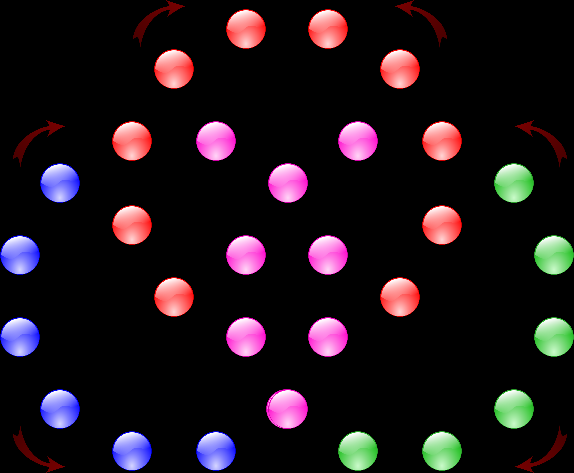
\includegraphics[width=1.0\linewidth]{figure01.png}
	\caption{The Fish Ring combinatorial puzzle in its ordered state}
	\label{figure01}
\end{figure}

Predefined sequences of actions are used to arrange the combinatorial puzzles. These sequences may be called by the more general name of ordering formulas. The most famous combinatorial puzzles are well-studied, and the formulas for their arrangement are well-known. In this context, the question arises: How do we discover such formulas for newly created puzzles or puzzles that still need to be thoroughly analyzed?

The present research proposes a way to explore combinatorial formulas that can be used to order the combinatorial puzzle called Fish Rings (Fig. \ref{figure01})\cite{Balabanov2015}.

The rest of the paper is organized as follows: The second section introduces the puzzle and its mechanics; The third section describes the practical implementation, in the form of program code, for the study of combinatorial formulas; The fourth section deals with the experimental part and the achieved results; The final section concludes and suggests further research.

\section{FISH RINGS PUZZLE}

The Fish Rings combinatorial puzzle emerged due to the concepts introduced in another widely known puzzle, the Hungarian Eight. In this puzzle type, colored balls are rolled into mechanically confined chutes; in both cases, the chutes are circular. Circular chutes typically have intersection points, allowing balls to move from one circle to another based on color. In the Fish Ring puzzle (Fig. \ref{figure01}), balls of four colors are utilized, housed in three circular chutes intersecting at six points. The rotation of balls in the three circles enables each ball to traverse between circles and land in any of them.

In the initial stages of the puzzle-solving process, minimal effort is required since most of it gets sorted out. The real challenge arises when the majority of the puzzle is already organized. This situation resembles the Rubik's Cube, where arranging the first two rows is relatively straightforward. However, the complexity intensifies when dealing with the already arranged pieces while arranging the base.

A formal grammar corresponding to the game can be defined for combinatorial puzzles. This formal grammar can be concise or expanded. The Fish Ring puzzle comprises three circles with spinning balls. By designating the top circle as A, the left circle as B, and the right circle as C, a minimal grammar for the Fish Ring puzzle involves these three Latin alphabet letters. Each letter signifies a counterclockwise rotation of the circle (clockwise is also implied). Using A, B, and C, sentences (formulas) can be constructed to reach any achievable game state. Minimal grammar serves as a robust mathematical formalism. However, more advanced variants of formal grammar are advisable for practical game usage.

An initial extension specifies the rotation direction, where +A, +B, and +C denote counterclockwise rotations, and -A, -B, and -C signify clockwise rotations. To condense sentences constructed with formal grammar, in addition to direction, numbers 1 to 9 may be applied to indicate the number of consecutive rotations of the corresponding circle. With these two extensions, the minimal formal grammar evolves into a more comprehensive set of symbols: -9A, -8A, -7A, -6A, -5A, -4A, -3A, -2A, -1A, +1A, +2A, +3A, +4A, +5A, +6A, +7A, +8A, +9A, -9B, -8B, -7B, -6B, -5B, -4B, -3B, -2B, -1B, +1B, +2B, +3B, +4B, +5B, +6B, +7B, +8B, +9B, -9C, -8C, -7C, -6C, -5C, -4C, -3C, -2C, -1C, +1C, +2C, +3C, +4C, +5C, +6C, +7C, +8C, +9C.

Choosing formal grammar also guides the search for suitable formulas contributing to the puzzle's arrangement in its final phases.

\section{PROGRAMMATIC IMPLEMENTATION}

Before the advent of computers, enthusiasts delved into combinatorial puzzles manually. Individuals attempted to arrange them to experiment with different sequences, seeking effective general solutions. This analytical process was time-consuming and marked by relatively high complexity \cite{Archer2007}. With the emergence of computer computation, such puzzles can now be analyzed with significantly greater comprehensiveness and within shorter time frames.

Modern computing technology facilitates the exploration of various formulas for shifting the puzzle. For this study, all possible formulas ranging from 1 command to 7 commands in length are generated. A complete exhaustion algorithm is applied\cite{Balabanov2024a}. Among the patterns generated, only those that move precisely two balls relative to the initial state of the puzzle are recorded. The focus lies on such formulas, as in the final phase of arranging the puzzle, sequences of commands preserving the already ordered part of the game would be most beneficial.

For generation purposes, the game is reconstructed as a model represented by one-dimensional arrays of numbers. Six circle rotation operations are implemented, and a simplified code fragment is created to perform syntactic and grammatical analysis of the submitted formulas according to the rules of the chosen formal grammar.

\section{EXPERIMENTS \& RESULTS}

All experiments were conducted on a computer with the following specifications: Asus-2023, featuring a 12th generation Intel(R) Core(TM) i7-12700 processor running at 2.10 GHz, 32 GB RAM, and a 64-bit operating system (x64-based processor). The specific operating system version used is Windows 11 Pro 23H2 22631.3007, and the software utilized for the experiments is Java(TM) SE Runtime Environment (build 19.0.2+7-44) Java HotSpot(TM) 64-Bit Server VM (build 19.0.2+7-44, mixed mode, sharing).

As a result of the performed calculations, 2,198,814 formulas were identified, meeting the conditions of having a length of 1 to 7 commands and displacing only two balls relative to the initial state of the puzzle\cite{Balabanov2024b}. The number of unique formulas is significantly less, as complete exhaustion generates sequences of the type -A+A, canceling each other out.

From this detailed list of formulas, one can manually select those offering the best prospect of ordering the puzzle in its final phase. Examples of such formulas include +3C+3B-3C-3B (Fig. \ref{figure02}) and -1C-4B+1C+4B (Fig. \ref{figure03}).

\begin{figure}
	\centering
	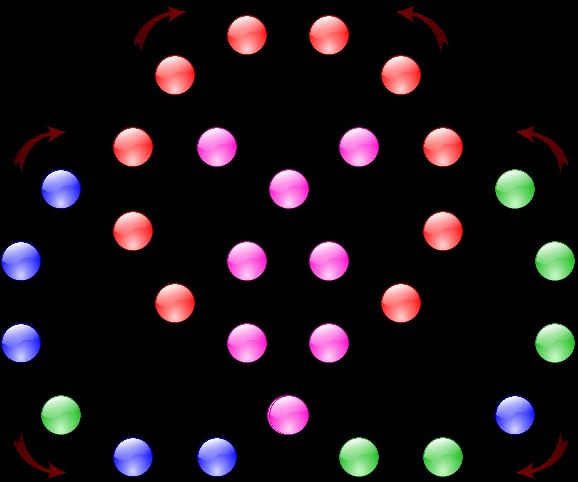
\includegraphics[width=1.0\linewidth]{figure02.png}
	\caption{Result of applying the formula +3C+3B-3C-3B}
	\label{figure02}
\end{figure}

\begin{figure}
	\centering
	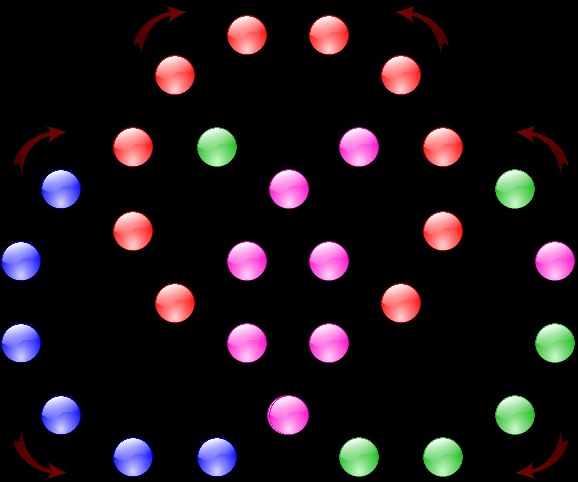
\includegraphics[width=1.0\linewidth]{figure03.png}
	\caption{Result of applying the formula -1C-4B+1C+4B}
	\label{figure03}
\end{figure}

In both formulas, it is evident that the displacement is precisely of two puzzle balls. A detailed analysis of the formulas is not performed, though necessary, as the balls are indistinguishable within their color group. The formula list may displace more than two items in multi-colored puzzle configurations.

\section{CONCLUSIONS}

The present research proposes a method to search for universal formulas in the arrangement of combinatorial puzzles. For the study's purposes, a digital model of the game in question and implemented commands to manipulate the individual elements of the puzzle were developed. To select suitable formulas for arranging the game in its final state, a list of formulas that met predetermined criteria was generated. The results indicate that this approach to solving combinatorial puzzles can be efficient and widely applicable.

Future research could explore other games within the combinatorial puzzles category. Additionally, experimenting with meta-heuristic algorithms for global optimization in the search for combinatorial puzzle arrangements could be considered.

\section{ACKNOWLEDGMENTS}

This work has been granted funding from the National Scientific fund program for COST actions support KP-06-KOST/23 and ...

\bibliography{references}
\bibliographystyle{eurosis}
\bibpunct[; ]{(}{)}{,}{a}{}{;}

\end{document}
